\subsection{Taylor-Couette Flow}

\subsubsection{Theoretical description}

\begin{figure}[!bp]
  \begin{minipage}[c]{0.6\textwidth}
      \centering
        \resizebox{0.9 \textwidth}{!}{
       \import{gfx/immersed_boundary/tcflow//}{tcsystem.pdf_tex}
      }
  \end{minipage}
  \begin{minipage}[c]{0.3\textwidth}
      \caption{Setup of the Poiseuille-flow channel.
      \label{validation:setup_pf}
      }
  \end{minipage}
\end{figure}

As a last test case for grid convergence studies we want to introduce the taylor-couette system.
The setup is exemplarly shown in Fig. (). It contains of two coaxial in z-direction oriented cylinders
with different radii $R_i$ and rotation rates $\Omega_i$. The fluid domain is given by the gap between the cylinders and
periodic in z-direction.\\
In dependency of the different domain paratemers different flow regimes can occur, criteria ...\\
We examine radial couette flow where the outter cylinder does not rotate ...\\
In constrast to the previously examined test cases this system provides different characteristics
of the flow regime at the fluid domain border. The flow along the borders is not orthogonal to the curvature of
the boundary like in the poiseuille flows we investigated before. Furthermore  new boundary
conditions are introduced, to be more precisely the Dirichlet condition is now given by $|\vec{v}(\vec{r})|_{r_i} | = |\Omega_i \times \vec{r}|$.
To begin with we want to examine the flow where the outer cyinder is not rotating, that is $\Omega_2 = 0$.
In literature this system is usually referred to as circular coutte flow (CCF) (CITE). Furthermore we want to investigate the flow regime
below the critical instability which means that $v_z=0$. In cylindrical coordinates the problem can be reduced to a two-dimensianol coordinate system with
the coordinates $(r, \phi)$, given by the coordinate transformations $x=r\cos(\phi), y = r\sin(\phi)$.
For the non-dimensionalization we choose the default convention (CITE) $x^*=x/(R_2 - R_1)$, $v^*=v/(R_1\Omega_1)$, $t^*=tR_1\Omega_1/(R_2-R_1)$ and $\rho^*=\rho$.
The flow is then characterized by the Reynolds number $Re = \frac{\Omega R_1d}{\nu}$. With this convention the equations of motion for the steady state are given by ()
\begin{align}
    -\frac{u^2_\phi}{r} = - \frac{\partial p}{\partial r}, 0 = \frac{1}{Re}\frac{\partial}{\partial r}\left(\frac{1}{r}\frac{\partial}{\partial r}(r u_\phi)\right)
\end{align}
Integrating the equations twice leads to the solution (CITE)
\begin{align}
    u_\phi = Ar + \frac{B}{r}
\end{align}
with
\begin{align}
    A = \frac{-\Omega_1R_1^2}{R^2_2 - R^2_1} ; B = \frac{\Omega_1R^2_1 R^2_2}{R^2_2 - R^2_1}
\end{align}

\subsubsection{Grid Convergence Study}

For the grid convergence study a reynolds number of $Re=50$  similar like in () was chosen in order to make sure the flow regime
is below the critical instability. With this exception all other parameters where kept the same like in section ().
The results of the computation are shown from Fig. () to Fig. ().


\clearpage
\begin{figure}[!bp]
  \begin{minipage}[c]{0.5\textwidth}
      \includegraphics{gfx/immersed_boundary/tcflow/theo/vp.pdf}
      \caption{Relative $l_2$-error for different Volume-Penalization methods.}
  \end{minipage}
  \begin{minipage}[c]{0.5\textwidth}
      \includegraphics{gfx/immersed_boundary/tcflow/theo/df.pdf}
      \caption{Relative $l_2$-error for different Direct-Forcing methods.}
  \end{minipage}
  \begin{minipage}[c]{0.5\textwidth}
      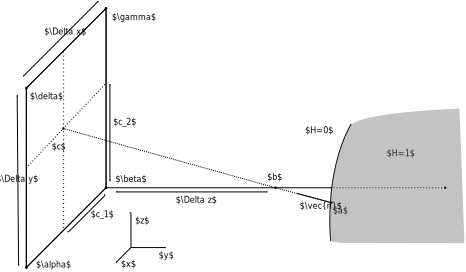
\includegraphics{gfx/immersed_boundary/tcflow/theo/ip.pdf}
      \caption{Relative $l_2$-error for different Interpolation methods.}
  \end{minipage}
  \begin{minipage}[c]{0.5\textwidth}
      \includegraphics{gfx/immersed_boundary/tcflow/theo/all.pdf}
      \caption{Relative $l_2$-error for the methods with the smallest error in comparsion.}
  \end{minipage}
\end{figure}
\clearpage


